\documentclass[a4paper,12pt]{report}
\usepackage{ctex}
%\usepackage{xeCJK}
\usepackage{times}
\usepackage{setspace}
\usepackage{fancyhdr}
\usepackage{graphicx}
\usepackage{wrapfig}
\usepackage{array}  
\usepackage{fontspec,xunicode,xltxtra}
\usepackage{titlesec}
\usepackage{titletoc}
\usepackage[titletoc]{appendix}
\usepackage[top=30mm,bottom=30mm,left=20mm,right=20mm]{geometry}
\usepackage{cite}
\usepackage{listings}
\usepackage[framed,numbered,autolinebreaks,useliterate]{mcode} % 插入代码
\usepackage{algorithm, algorithmic} %伪代码
\XeTeXlinebreaklocale "zh"
\XeTeXlinebreakskip = 0pt plus 1pt minus 0.1pt

%---------------------------------------------------------------------
%	页眉页脚设置
%---------------------------------------------------------------------
\fancypagestyle{plain}{
	\pagestyle{fancy}      %改变章节首页页眉
}

\pagestyle{fancy}
\lhead{\kaishu~生物智能与算法报告~}
\rhead{\kaishu~21721164~胡亮~}
\cfoot{\thepage}

%---------------------------------------------------------------------
%	章节标题设置
%---------------------------------------------------------------------
\titleformat{\chapter}{\centering\zihao{-1}\heiti}{\chinese{chapter}}{1em}{}
\titlespacing{\chapter}{0pt}{*0}{*6}

%---------------------------------------------------------------------
%	摘要标题设置
%---------------------------------------------------------------------
\renewcommand{\abstractname}{\zihao{-3} 摘\quad 要}

%---------------------------------------------------------------------
%	参考文献设置
%---------------------------------------------------------------------
\renewcommand{\bibname}{\zihao{2}{\hspace{\fill}参\hspace{0.5em}考\hspace{0.5em}文\hspace{0.5em}献\hspace{\fill}}}

%---------------------------------------------------------------------
%	引用文献设置为上标
%---------------------------------------------------------------------
\makeatletter
\def\@cite#1#2{\textsuperscript{[{#1\if@tempswa , #2\fi}]}}
\makeatother

%---------------------------------------------------------------------
%	目录页设置
%---------------------------------------------------------------------
\titlecontents{chapter}[0em]{\songti\zihao{-4}}{\thecontentslabel\ }{}
{\hspace{.5em}\titlerule*[4pt]{$\cdot$}\contentspage}
\titlecontents{section}[2em]{\vspace{0.1\baselineskip}\songti\zihao{-4}}{\thecontentslabel\ }{}
{\hspace{.5em}\titlerule*[4pt]{$\cdot$}\contentspage}
\titlecontents{subsection}[4em]{\vspace{0.1\baselineskip}\songti\zihao{-4}}{\thecontentslabel\ }{}
{\hspace{.5em}\titlerule*[4pt]{$\cdot$}\contentspage}


\begin{document}
%---------------------------------------------------------------------
%	封面设置
%---------------------------------------------------------------------
\begin{titlepage}
	\begin{center}
		
    
\includegraphics[width=0.9\textwidth]{pic//zju.jpg}\\
    \vspace{10mm}
    \textbf{\zihao{2}\kaishu{计算机科学与技术学院}}\\[0.8cm]
    \textbf{\zihao{2}\kaishu{ 生物智能与算法报告}}\\[3cm]
    
	\vspace{\fill}
	
\setlength{\extrarowheight}{3mm}
{\songti\zihao{3}	
\begin{tabular}{rl}
	
	% {\makebox[4\ccwd][s]{班\qquad 级:}}& ~\kaishu 通信二班\\
	
	{\makebox[4\ccwd][s]{姓\qquad 名:}}& ~\kaishu 胡亮 \\ 

    {\makebox[4\ccwd][s]{学\qquad 号:}}& ~\kaishu 21721164 \\ 
   
	{\makebox[4\ccwd][s]{老\qquad 师:}} & ~\kaishu 袁昕 \\ 


\end{tabular}
 }\\[2cm]
\vspace{\fill}
\zihao{4}
2017\textasciitilde 2018春学期\\
使用\LaTeX 撰写于\today
	\end{center}	
\end{titlepage}

%---------------------------------------------------------------------
%  摘要页
%---------------------------------------------------------------------
\begin{abstract}
\begin{spacing}{1.5}
	{\zihao{-4}
	作为一种新型的群体智能算法,人工蜂群算法自从提出以来就受到了广泛的关注,并涌现大量的研究成果。本文首先介绍了人工蜂群算法的起源,然后详细地介绍了人工蜂群算法的生物背景、算法原理和实现步骤,最后说明近年来对人工蜂群算法的比较、改进和应用领域,并进一步提出了未来要改进的方向。\\[0.5cm]
	\textbf{关键字}:\quad 人工蜂群算法 \quad 群体智能 \quad 觅食行为
	}
\end{spacing}
\end{abstract}

%---------------------------------------------------------------------
%  目录页
%---------------------------------------------------------------------
\tableofcontents % 生成目录


\chapter{引言}
\setcounter{page}{1}

\begin{spacing}{1.5}
	人工蜂群算法(artificial bee colony,ABC)是由土耳其埃尔吉耶斯大学学者Karaboga于2005年提出,其基本思想是启发于蜂群通过个体分工和信息交流,相互协作完成采蜜任务。与传统的优化方法相比,它的主要优点是不需要了解问题的特殊信息,只需要对问题进行优劣比较,通过各个人工蜂群个体的局部寻优行为,最终在群体中使得全局最优值凸现出来,具有较快的收敛速度。但同时也存在以下问题:ABC算法存在“早熟”的收敛性缺陷,即在接近全局最优解时,已陷入局部最优。

\end{spacing}

\chapter{人工蜂群算法}
\begin{spacing}{1.5}
\songti\zihao{-4}

\section{自然界的蜂群}
		蜜蜂是一种社会性群居性动物,虽然单个蜜蜂的行为简单,但群体却表现出极其复杂的智慧行为。自然界的蜜蜂能在各种环境下,以极高的效率从食物源(花朵)中采集蜂蜜,同时还能适应环境的改变。

		蜂群实现群体智能的最小搜索模型包括三个基本要素:蜜源、雇佣蜂(Employed Foragers)和未被雇佣蜂(Unemployed Foragers)和两种基本行为:为蜜源招募蜜蜂(Recruit)和放弃蜜源(Abandon)。其中雇佣蜂又被称为引领蜂(leader),引领蜂与其所采集的蜜源一一对应,存储着该蜜源的相关信息。被雇佣蜂又分为跟随蜂(onlooker)和侦查蜂(scouter),跟随蜂等在蜂巢中通过引领蜂分享的信息采集花蜜,侦查蜂负责搜索新的蜜源。在群体智慧的形成过程中,蜜蜂间交换信息是最重要的一环。生物学家发现蜜蜂以跳舞的形式来交换信息,而蜂巢中舞蹈区是最重要的信息交换地,蜜源的信息在舞蹈区通过摇摆舞的形式与其他蜜蜂共享。

			\begin{figure}[tbp]
				\centering
				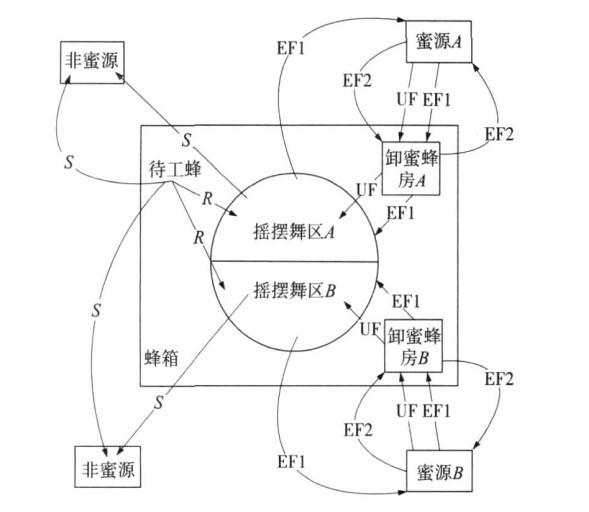
\includegraphics[width=0.6\textwidth]{pic/bee4.jpg}
				\caption{蜜蜂的搜索行为}
				\label{fig:pt1}
			\end{figure}

		蜜蜂对蜜源的搜索行为简单描述如下:初始时蜜蜂以侦查蜂的身份搜索,其搜索过程可由系统初始经验决定,也可完全随机。经过一轮侦查后,当蜜蜂找到蜜源后,此时蜜蜂变成引领蜂,并根据自己的能力记住蜜源的信息(位置、花蜜的质量等),每一只引领蜂与自己找到蜜源一一对应。如图2.1所示,蜜蜂在采蜜结束后回到蜂巢,将有以下选择:
			\begin{itemize}
				\item {在舞蹈区进行蜜源信息分享后,发现自己的蜜源质量并不高,放弃蜜源重新变成侦查蜂寻找新蜜源(图中UF线)}
				\item {在舞蹈区跳舞招募蜜蜂,此时蜂巢里的非雇佣蜂以一定概率跟随引领蜂回到蜜源进行采蜜(图中EF1线)}
				\item {继续会蜜源采蜜而不进行招募(图中EF2)}
			\end{itemize}
		而蜂巢里的非雇佣蜂也有如下选择:
			\begin{itemize}
				\item {以侦查蜂的身份,自发搜索蜂巢附近的蜜源(图中S线)}
				\item {在观察完摇摆舞被雇佣成为跟随蜂,开始搜索对应蜜源附近并采蜜(图中R线)}
			\end{itemize}

\section{算法模型与原理}
	ABC算法是模拟蜜蜂采蜜过程而提出来的群体智能算法,其首度提出即是用于解决连续函数的求解问题,其后更是广泛应用于优化问题的求解,如表2.1,ABC算法在求解优化问题时,蜜源的位置被抽象成解空间的一个点,蜜源的质量对于解的适应度fit,寻找和采集蜜源的过程即优化问题的求解过程;另外,蜜源的最大质量即优化问题的最优解。

	\begin{table}[!htbp]
		\centering
		\caption{采蜜行为与优化算法的映射关系}
		\label{my-label}
		\begin{tabular}{|c|c|ccc}
		\cline{1-2}
		采蜜行为    	& 优化问题 	&  &  &  \\ \cline{1-2}
		蜜源位置		& 可行解   	&  &  &  \\ \cline{1-2}
		蜜源质量 		& 适应度 	&  &  &  \\ \cline{1-2}	
		采蜜速度 		& 收敛速度  &  &  &  \\ \cline{1-2}
		蜜源最大质量 	& 最优解 	&  &  &  \\ \cline{1-2}
		\end{tabular}
	\end{table}

	其中角色转换是ABC算法特有的机制,蜂群通过引领蜂、跟随蜂和侦查蜂三类角色的转换,从而共同协作寻找高质量的蜜源。在ABC算法搜索优良解的过程中,3类蜜蜂的作用有所差别:引领蜂用于维持优良解(记录当前局部最优解);跟随蜂用于提高收敛速度(搜索局部最优解的附近空间);侦查蜂用于增强摆脱局部最优的能力(全局搜索)。
		\begin{figure}[htbp]
			\centering
			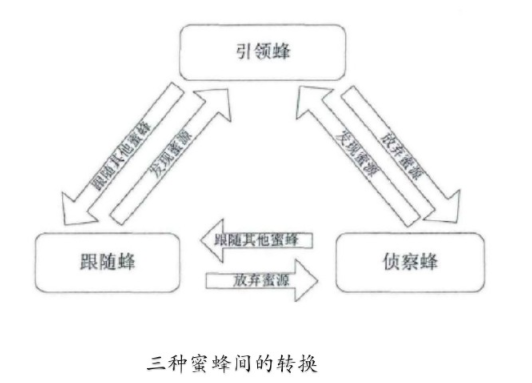
\includegraphics[width=.6\textwidth]{pic/bee5.png}
			\caption{角色转换}
			\label{fig:pt2}
		\end{figure}

\section{算法步骤}

		人工蜂群算法的主要实现步骤包括初始化种群、循环、引领蜂阶段、跟随蜂阶段、侦查蜂阶段、记录当前最优解和循环结束输出全局最优解,先对各实现步骤具体介绍,可得详细内容如下:

		{\bfseries 初始化种群} \quad 设解空间的维度为D,初始蜜源的个数为NP,控制参数limit(局部搜索次数)和最大循环数MaxCycle等,将蜂群分为引领蜂、侦查蜂、跟随蜂三个类型,且引领蜂和跟随蜂各占蜂群的一半,数量等于NP,并根据(2.1)(2.2)式在搜索空间随机产生NP个蜜源,并为每一个蜜源分配一个引领蜂。
			\begin{equation}
				X_{i} = [ x_{i1},x_{i2},\cdots,x_{iD}]
			\end{equation}
			\begin{equation}
				x_{id} = L_{d} + rand(0,1) * (U_{d} - L_{d})
			\end{equation}

			$L_{d},U_{d}$分别是解空间的上限和下限。

		{\bfseries 引领蜂阶段} \quad 在搜索的开始阶段,引领蜂计算其对应蜜源的适应度,如(2.3)式所示。再在蜜源i的附近根据(2.4)式搜索一个新的蜜源(一次搜索),当新蜜源的适应度fit(vi)优于xi时,采用贪婪选择方法用新蜜源替代原来的蜜源,否则保留Xi。当所有的引领蜂完成贪婪选择后,飞回到蜂巢舞蹈区进行交流。
			\begin{equation}
				fit_{i} = \left\{  
	             		\begin{array}{lr}  
	             			1 / (1 + f_{i}),f_{i} \leq 0 &  \\  
	             			1 + abs(f_{i}), otherwise    
	             		\end{array}  
	           		\right.
			\end{equation}
			\begin{equation}
				v_{id} = x_{id} + \varphi * (x_{id} - x_{jd})
			\end{equation}

			其中(2.3)式中$f_{i}$表示解的函数值,(2.4)式中$ j \neq i $,表示在NP个蜜源中随机选择一个不等于i的蜜源;$ \varphi $是[-1,1]均匀分布的随机数。

		{\bfseries 跟随蜂阶段} \quad 跟随蜂根据引领蜂分享的蜜源信息,按式(2.5)的方式计算概率并选择跟随,并采用如2一样的贪婪选择方法在所对应的蜜源附近搜索局部最优解。
			\begin{equation}
				p_{i} = fit_{i} / \sum_{i=1}^{NP} fit_{i} 
			\end{equation}

		{\bfseries 侦查蜂阶段} \quad 在搜索过程中,若蜜源Xi经过多次搜索达到局部搜索阈值limit而未找到更好的蜜源,则该蜜源会被放弃,与之对应的引领蜂会变成侦查蜂,如(2.6)式所示重新在全局空间随机搜索一个新的蜜源代替Xi。
			\begin{equation}
				X_{i}^{t+1} = \left\{  
			             		\begin{array}{lr}  
			             			L_{d} + rand(0,1) * (U_{d} - L_{d}),t_{i} \geq limit &  \\  
			             			X_{i}^{t}, otherwise    
			             		\end{array}  
			              \right. 
			\end{equation}

		{\bfseries 算法终止} \quad 记录当前所有蜜蜂找到的最优蜜源,并跳至第2步,直到满足最大迭代次数MaxCycle或者小于优化误差时,输出全局最优解。

		算法伪代码如下:
		\begin{algorithm}[H]
		\caption{ABC}\label{bee_alg}
		\algsetup{linenosize=\tiny} \scriptsize
			\begin{algorithmic}
				\STATE{Initialize the food sources $X_i(i=1,2,3,...,n)$ by Eq.1,\\ 
				the colony count,NP; control parameter,limit; the Max cycle count, MaxCycle;}
				
				\FOR {cycle from 1 to MaxCycle do}
					\FOR {each employee bee i do}
						\STATE {Choose a food source $X_{k}$ in the neighbourhood of $X_{i}$; }
						\STATE {select a jth dimension above all dimension;}
						\STATE {Genernate a food source vi in the neighborhood of $x_{i}$ and $x_{k}$ by Eq.2;}
						\STATE {Apply greedy selection between of $x_{i}$ and $x_{k}$;}
					\ENDFOR
					\FOR {each onlooker bee i do}
						\STATE {select a food source $X_{i}$ depending on probability pi using Eg.3; }
						\STATE {Choose a food source $X_{k}$ in the neighbourhood of $X_{i}$; }
						\STATE {Genernate a food source vi in the neighborhood of $x_{i}$ and $x_{k}$ by Eg.2;}
						\STATE {Apply greedy selection between of $x_{i}$ and $x_{k}$;}
					\ENDFOR
					\IF {there exits an abondoned food source}
						\STATE {Scout bee determines a new food source by Eq.1; }
					\ENDIF
					\STATE {Update best food source;}
				\ENDFOR
			\end{algorithmic}
		\end{algorithm}

\end{spacing}

%---------------------------------------------------------------------
%  第二节
%---------------------------------------------------------------------
\chapter{研究与改进}

\begin{spacing}{1.5}
\section{比较}
	人工蜂群算法最初是为了解决数值问题而提出并形成的,这就使得研究目的即设定为和其他著名的算法进行比较,例如粒子群算法PSO、差分进化算法DE和实数编码遗传算法RCGA等。我们采用如下4个基准函数对算法进行优化测试:
	
	\begin{table}[!htbp]
		\centering
		\caption{Numerical benchmark function}
		\label{my-label}
		\begin{tabular}{|c|c|c|cc}
		\cline{1-2}
		Name     		& function  														& range 		&  &  \\ \cline{1-3}
		Sphere函数 		& $f_{1}(x)= \sum_{i=1}^d x_{i}^2 $     							& [-100,100]	&  &\\ \cline{1-3}
		Rosenbrock函数	& $f_{2}(x)= \sum_{i=1}^d (100(x_{i+1}-x_{i}^2)^2 + (x_{i} - 1)^2 ) $ 	& [-30,30] 		&  &  \\ \cline{1-3}
		Griewank函数    	& $f_{3}(x)= \frac{1}{4000} \sum_{i=1}^d x_{i}^2 -  \prod_{i=1}^d cos(\frac{x_{i}}{\sqrt{i}}) + 1 $   	& [-600,600]	&  &  \\ \cline{1-3}
		Rastrigin函数   	& $f_{4}(x)=\sum_{i=1}^d (x_{i}^2 - 10cos(2   \pi 2 x_{i} + 10)$     	& [-5.12,5.12] 	&  &  \\ \cline{1-3}
		\end{tabular}
	\end{table}

其中函数 $ f_{1}(x) $是单峰函数; 函数 $ f_{2}(x) $ 是很难极小化的病态函数; 函数 $ f_{3}(x) $, $ f_{4}(x) $都是具有大量局部最优点的多峰函数,式中d为变量维度,取d=30;4个个基准测试函数的全局极小值均为$ minf_{i}(x) = 0$。 为验证 ABC 算法的优化性能,将其与常用的几种全局优化算法 RCGA,PSO,DE进行了比较。算法的参数设置如下: 群体规模 N = 50,迭代次数 tmax = 2000。

将上述4种不同算法对4个基准测试函数分别独立运行50次后将最优解取平均值,并计算最优化结果的标准差,结果如表所示。可以看出ABC算法除了$f_{3}$优化结果比DE算法稍差外,其他函数优化结果均优于其他几种算法。
		\begin{figure}[htbp]
			\centering
			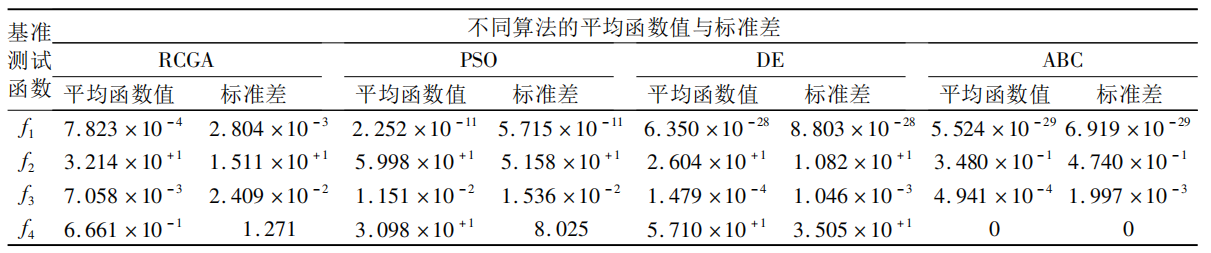
\includegraphics[width=1.0\textwidth]{pic/bee10.png}
			\caption{四种算法运行平均最优值比较}
			\label{fig:pt3}
		\end{figure}

下图为采用 RCGA,PSO,DE 和ABC对4个基准测试函数独立运行50次,平均最小函数值随迭代次数的变化过程曲线。由下图可以看出,ABC算法和其他几种算法相比不但具有很强的全局搜索能力,而且具有较快的收敛速度,其优化性能大大优于同类的PSO算法。
		\begin{figure}[htbp]
			\centering
			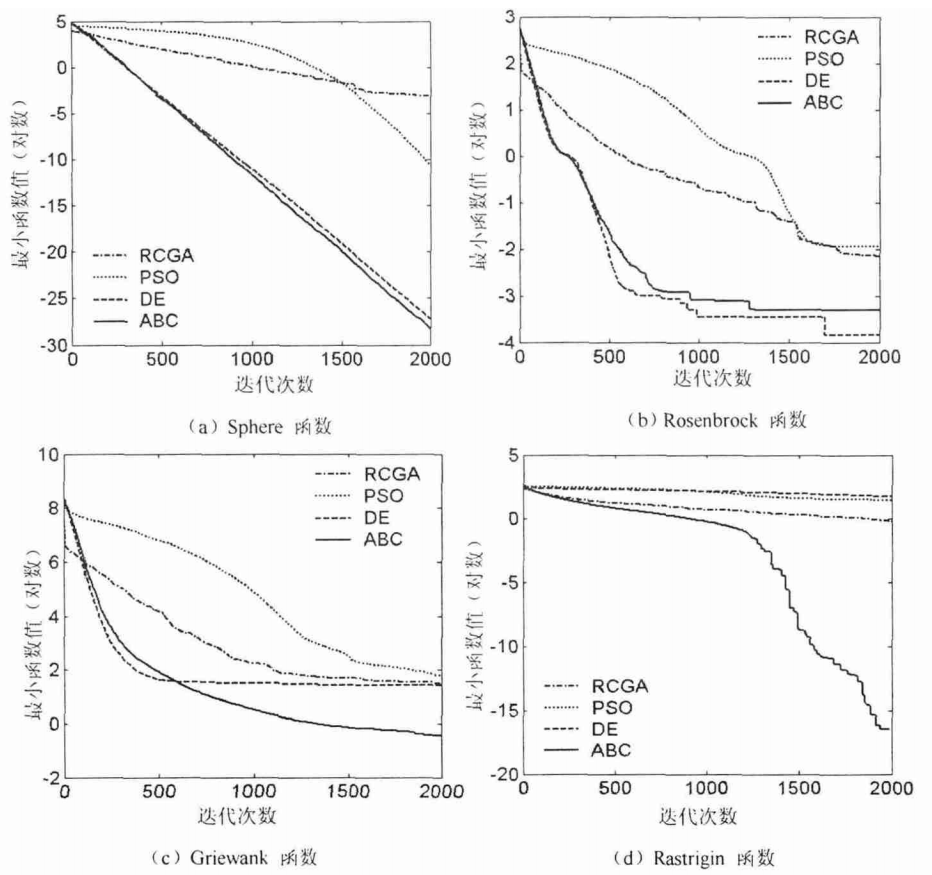
\includegraphics[width=0.6\textwidth]{pic/bee11.png}
			\caption{四种算法测试最小数随迭代次数的变化过程曲线}
			\label{fig:pt4}
		\end{figure}

\section{改进}
	ABC算法虽然控制参数少,实现简洁且在实现某些复杂问题上颇具优势,但随着迭代搜索接近尾声,蜂群个体的多样性及搜索速度会逐渐降低,而种群整体出现早熟收敛、陷入局部极值的可能性却显著提高。针对ABC算法的不足,国内外的学者提出了很多改进方法,研究成果简单归纳为混合算法、对搜索机制的改进和其他环节的改进等。

	文献[5]结合混沌映射、鲶鱼效应形成一个新的混合算法-基于混沌鲶鱼效应的人工蜂群算法,该算法将混沌映射、鲶鱼效应结合到ABC算法中去,以此提高种群的搜索速率和增强个体跳出局部最优解的能力。该算法一方面通过使用混沌映射的方法替代原来的一般随机化初始蜜源过程;另一方面,将鲶鱼效应施加到蜜蜂种群内,并以混沌波动的方式衍生出一种新型的混沌鲶鱼蜂,用来替代原侦查蜂负责搜索新蜜源的任务,且同原蜂群个体之间形成了有效的竞争、协作机制。针对ABC搜索机制的改进,大部分优化都集中在式(4)寻找邻域新的蜜源,该公式适宜探索,但不适合搜寻新蜜源,导致收敛速度过慢;有的学者采用局部随机搜索算子对当前最优蜜源进行局部搜索,以加快搜索速度,同时利用基于排序的选择概率替代原算法中直接利用适应度计算的概率,来保证解的多样性。

\section{应用}
	最早的人工蜂群算法是用来解决数值问题,其后来的研究成果已经用来解决离散与连续问题,现在已经将ABC算法应用到多个研究领域:神经网络训练,组合优化,无线传感网等多个领域。有的学者将ABC算法应用于前馈神经网络的训练,甚至还用于优化神经网络的结构、连接权重和激励函数等。其中应用最成功的还是组合优化领域。

	经典的优化算法一般很难求解组合优化问题,而ABC算法在旅行商问题、生产调度、项目调度和背包问题等组合优化问题中都有成功应用,我们在这里可以用人工蜂群算法用于求解旅行商问题(TSP),旅行商问题可以简单地描述为:给定N个城市C=(C1,C2,…CN),求一条从一个城市出发拜访N个所有城市的道路(Cn1,Cn2,…CnN),且每个城市有且只能访问一次,最终回到开始的城市,其中任意两个城市的距离为d(Ci,Cj),使得求得的路径距离最小。

	所有城市的任一种排列即是问题解空间的一个解,因此初始解空间就是N个城市的排列组合。在人工蜂群算法中,将城市个数N作为蜜源的维度,每一个蜜源的位置表示其中一个路径的组合,用这条路径的距离长度表示蜜源的适应度,也就是说,适应度越小的蜜源,所表示的路径也就最优。引领蜂和跟随蜂在更新蜜源位置时,是选择其位置对应的路径任意两处进行调换生成新的路径,表示新的位置。

	ABC求解TSP问题步骤类似上面框架,只是在初始化阶段和更新阶段分配和更新道路,为验证算法的有效性,利用仿真实验测试ABC算法在TSP上的性能,城市个数设为14,初始化蜜蜂种群数为NP=20,最大搜索次数limit为100,最大迭代次数MaxCycle为2500;如图所示,左图是初始路径图,从1按序排到14,经过2500次迭代后得到的最优路径为(1,2,14,3,4,5,6,12,7,13,8,11,9,10,1),其最优路径长度为30.8785;其长度的优化过程如图所示,初始时路径长度最高,经过700多次的迭代后已寻找到最优路径。


		\begin{figure}[htb]
		\begin{minipage}[b]{0.5\linewidth}
		\centering
		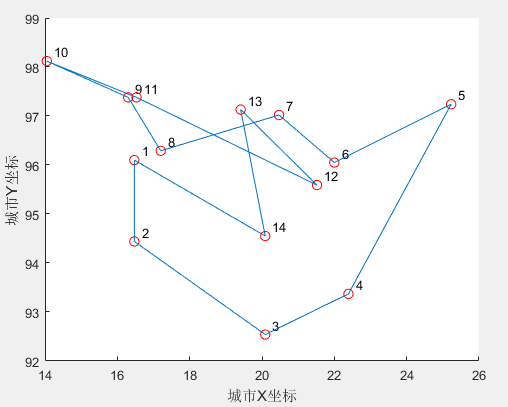
\includegraphics[width=2.5in,height=2.5in]{pic/bee7.png}
		\caption{初始路径图}
		\label{F4-5}
		\end{minipage}
		\begin{minipage}[b]{0.5\linewidth}
		\centering
		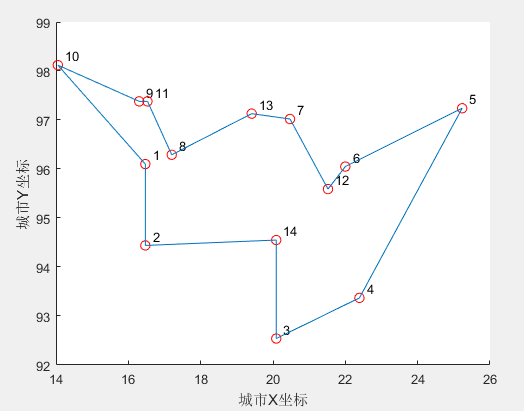
\includegraphics[width=2.5in,height=2.5in]{pic/bee8.png}
		\caption{结果路径图}
		\label{F4-6}
		\end{minipage}%
		\end{figure}

		\begin{figure}[htbp]
			\centering
			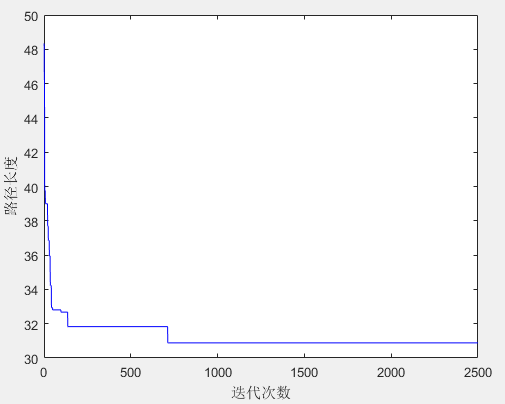
\includegraphics[width=.8\textwidth]{pic/bee9.png}
			\caption{优化曲线}
			\label{fig:pt3}
		\end{figure}

\end{spacing}


\chapter{结语}

\begin{spacing}{1.5}
	作为群体智能的一种,ABC算法与其他群体算法有着很多相似之处,比如都利用系统性,利用群体的概念表示解空间的个体集合,通过个体之间信息共享、相互协作完成迭代优化寻找最优解等任务。但人工蜂群算法也有一些独有特点,其中突出的一点是角色转换机制,在进行全局搜索的同时,也在进行局部搜索,同时还有跳出局部最优的能力,借此角色转换的机制,使得算法性能得到显著提升。

	人工蜂群算法自从提出以来,就受到了很多学者的关注,但总体来说,对ABC算法的研究还处于初级阶段,还有很多问题有待进一步的研究,简单归纳如下几点:
	
	理论研究:目前的研究大多围绕在算法的改进和应用上,而对ABC 算法的理论研究匮乏,从理论上无法剖析算法的行为。对于 ABC 的运行时间和收敛属性、适应值曲面和动态特性的理论研究还需进一步开展。

	参数设置:参数的合理设置对算法性能有着显著影响,现有的参数设置都是基于经验的,对具体问题和环境有很大依赖。研究 ABC 算法参数选取方法,尤其是如何设置具有普适性的无须精密调节的参数及自适应参数的研究及相关理论支持值得开展。
		
	应用领域:进一步扩展人工蜂群算法的应用领域,研究ABC算法在多目标、多约束、离散和动态的不确定的智能优化问题和动态优化问题等。

\end{spacing}

%---------------------------------------------------------------------
%  参考文献设置
%---------------------------------------------------------------------
\addcontentsline{toc}{chapter}{参考文献}

\begin{thebibliography}{99}
\songti \zihao{-4} 	

	\bibitem{bee_bib1} 何尧,刘建华,杨荣华.人工蜂群算法研究综述[J/OL].计算机应用研究,2018(05):1-8
	\bibitem{bee_bib2} 陈阿慧,李艳娟,郭继峰.人工蜂群算法综述[J].智能计算机与应用,2014,4(06):20-24
	\bibitem{bee_bib3} Karaboga D. An idea based on honey bee swarm for numerical optimization[R]. Technical report-tr06, Erciyes university, engineering faculty, computer engineering department, 2005.
	\bibitem{bee_bib4} 王慧.人工蜂群算法的性能比较研究[J].河北工程技术高等专科学校学报,2015(01):41-44.
	\bibitem{bee_bib5} 王生生,杨娟娟,柴胜.基于混沌鲶鱼效应的人工蜂群算法及应用[J].电子学报,2014,42(09):1731-1737.
	\bibitem{bee_bib6} 黄秋菀, 王志刚, 夏慧明. 求解旅行商问题的人工蜂群算法 [J]. 价值工程,2013,32(09):206-207
	
\end{thebibliography}


\end{document}